%%%%%%%%%%%%%%%%%%%%%%%%%%%%%%%%%%%%%%%%%
%ِ Assignment Supervisor: Dr.Abdullah Alharbi 
% Subject : Programming Language 
% Student Name: Abdullah Ahmad Alzahrani
% Student ID: 441015535
% Student E-mail: s441015535@st.uqu.edu.sa
%%%%%%%%%%%%%%%%%%%%%%%%%%%%%%%%%%%%%%%%%

%----------------------------------------------------------------------------------------
%	PACKAGES AND OTHER DOCUMENT CONFIGURATIONS
%----------------------------------------------------------------------------------------

\documentclass[11pt]{Abdullahmad} % Font size 

%----------------------------------------------------------------------------------------
%	TITLE SECTION
%----------------------------------------------------------------------------------------

\title{\textbf{SWIFT  Programing Language} \\ {\Large\itshape Apple Developer }} % Title and subtitle

\author{\textbf{Abdullah Ahmad Alzahrani} \\ \textit{441015535}} % Author and institution

\date{\today} % Date

%----------------------------------------------------------------------------------------

\begin{document}

\maketitle % Print the title section

%----------------------------------------------------------------------------------------
%	ABSTRACT AND KEYWORDS
%----------------------------------------------------------------------------------------


\begin{abstract}
This report provides an overview of the SWIFT programming language developed by Apple Inc. SWIFT is a modern programming language that is designed to be safe, fast, and interactive. It is used to develop applications for Apple's operating systems, including iOS, macOS, watchOS, and tvOS. The report highlights the key features of the language, including its syntax, data types, and control structures. It also discusses the benefits of using SWIFT for application development, such as improved safety, better performance, and reduced development time. Additionally, the report covers the various tools and resources available to developers using SWIFT, including Xcode, Playground, and Swift Package Manager. Overall, this report aims to provide a comprehensive understanding of the SWIFT programming language and its role in modern application development \cite{Goodwill2015}.
\end{abstract}

\hspace*{3.6mm}\textit{Keywords:} Swift, Apple, iOS, MacOS, WatchOS, tvOS % Keywords

\vspace{30pt} % Vertical whitespace between the abstract and first section

%----------------------------------------------------------------------------------------
%	ESSAY BODY
%----------------------------------------------------------------------------------------
\newpage
\section*{Introduction}

The development of mobile systems and applications requires appropriate programming languages and development tools. First, Objective-C was the primary language for iOS. In recent years, that Objective-C has been shown to cease
to meet modern developments\cite{7476687}.That's why Apple has begun to develop the new Swift programming language. It is a compiled programming language for iOS, watchOS, tvOS, macOS, and Linux applications. It was created for more; comfortable and safer code creation, but also easier learning programming. It is first introduced at Apple’s 2014 Worldwide Developers Conference. Language has undergone dynamic development, and this has occasionally led to problems. Swift brings simpler syntax, shorter code, and safer programs. The language is not a purely object-oriented language but is hybrid. Apple says that Swift is 2.6x faster than Objective-C and 8.4x faster than Python. Swift, together with Kotlin, is one of the fastest-growing programming languages \cite{doi:10.1137/1.9781611972764.5}.

%------------------------------------------------

\section*{Developing the history of the language (Year, People, House, Environment}

The Swift programming language was originally developed under the  guidance of  Chris Lattner at Apple, Inc. and first announced alongside  iOS 8 at Apple’s  Worldwide Developer Conference in 2014.
Though the primary goal of Swift has always been to make it easier to develop apps for Apple’s range of operating systems (iOS, macOS, tvOS,  watchOS, etc.), the Swift language and compilers  are open-source and available for use on a wide  range of other operating systems.

\begin{wrapfigure}{l}{0.42\textwidth} % Inline image example, use an 'r' column type to position the figure on the right
	
\includegraphics[width=\linewidth]{Apple.jpg}
	\caption{Apple Inc.}
\end{wrapfigure}
On the other hand, Swift is a relatively new programming language  designed specifically to make  programming  easier, faster, and less prone  to programmer error. Starting with a clean slate and no burden of  legacy, 
Swift is a new and innovative language with which to develop  applications. Thankfully, much of the syntax will be familiar to those  who have experience with other programming languages, such as C, C++, Java, and Kotlin


%------------------------------------------------
\newpage
\section*{Domain and Category of the Programming Langugae (SWIFT)}

The SWIFT programming language is primarily used for developing applications for Apple's ecosystem,
including macOS, iOS, watchOS, and tvOS. Therefore, its domain would be considered as 
mobile app development and software development for Apple's operating systems.
In terms of categories, SWIFT is an object-oriented programming language and is classified 
as a high-level language, which means it is designed to be easily read and written by humans, 
with a syntax that is closer to natural language than low-level languages like assembly. 
It is also a compiled language, meaning that the code is translated into machine-readable
instructions before being executed, rather than being interpreted at runtime.



%------------------------------------------------

\section*{Goals, Concerns, Success and Contributions of SWIFT apple programming Language}

Goals :
\begin{itemize}
	\item To make programming more approachable and accessible to beginners and experts alike.
	\item To make programming more efficient and less error-prone.
	\item To provide developers with a powerful, flexible, and modern programming language that is suitable for a wide range of applications and platforms.
        \item To create a language that is safe, fast, and interactive, allowing developers to build
      secure and efficient applications quickly and easily \cite{miller2001swift}.
\end{itemize}

Concerns :
\begin{itemize}
	\item Initially, one of the main concerns with SWIFT was that it was a new  programming
      language, and there was a risk that it would not be widely adopted by developers.
	\item Another concern was that there was a lack of documentation and resources 
      available when SWIFT was first released, which made it more challenging for
      developers to learn and use the language.
\end{itemize}

Success :
\begin{itemize}
	\item SWIFT has been widely adopted by developers and is now one of the most popular
       programming languages in the world.
	\item It has become the go-to language for iOS app development, and many popular apps, such 
       as Airbnb, Lyft, and LinkedIn, are built using SWIFT.
	\item SWIFT has also helped to simplify and streamline the development process, reducing the time
       and effort required to build high-quality applications.
        \item The language has also improved the safety and security of software development, 
       thanks to its strong type system, automatic memory management, and error-handling mechanisms
\end{itemize}

Contributions :
\begin{itemize}
	\item SWIFT has contributed significantly to the development of the Apple ecosystem, enabling
       developers to create high-quality applications for various platforms, including iOS, macOS, 
       watchOS, and tvOS.
	\item The language has also helped to advance the state of modern programming by introducing 
       new features and concepts, such as optionals, closures, and generics.
	\item SWIFT has also inspired other programming languages, such as Kotlin, which is now the 
       preferred language for Android app development.
\end{itemize}


%------------------------------------------------

\section*{What is a special or a new in the SWIFT programming Language.}

SWIFT introduced several new and innovative features that set it apart from other programming languages. Here are some of the most significant ones: \cite{singh2017raising}
\begin{enumerate}
	\item Safety and Security: SWIFT was designed with safety and security in mind. It uses a strong 
      type system that ensures that data is always handled correctly and prevents common
      programming errors such as null pointer exceptions. It also features automatic memory 
      management, which helps to prevent memory-related bugs and vulnerabilities.
	\item Optionals: Optionals are a unique feature in SWIFT that allows developers to handle the
      absence of a value. This feature helps to prevent runtime crashes caused by null pointer
      exceptions.
        \item Closures: Closures are a powerful feature in SWIFT that allows developers to write code in a
      more concise and expressive way. Closures are self-contained blocks of code that can be 
      passed around as variables and used to perform tasks such as sorting and filtering.
	\item Generics: Generics are another powerful feature in SWIFT that allows developers to write code 
    that is more flexible and reusable. Generics allow developers to create functions, classes,
    and data types that can work with any type of data.
	\item Playgrounds: SWIFT includes a feature called Playgrounds, which allows developers to test their 
   code in real-time and see the results immediately. Playgrounds are an excellent tool for learning
   and experimenting with SWIFT.
	\item Interoperability: SWIFT was designed to be interoperable with Objective-C,  which is the primary
   programming language used to develop macOS and iOS applications. This feature makes it easier
   for developers to integrate SWIFT code into existing Objective-C projects. \cite{garcia2015swift}
\end{enumerate}


%------------------------------------------------
\newpage
\section*{Overview of the SWIFT Apple programming language, including Examples
 and Description of major parts or commands of the SWIFT Apple 
programming language}

SWIFT is a powerful, modern, and open-source programming language developed by Apple Inc. 
It is designed to be safe, fast, and interactive, making it ideal for developing software applications
for various platforms, including iOS, macOS, watchOS, and tvOS. Here is an overview of SWIFT, 
including some examples and descriptions of its major parts or commands \cite{10006854}:

\begin{itemize}
	\item Variables and Constants: In SWIFT, you can declare variables and constants to store data. 
   A variable is a mutable value that can be changed, whereas a constant is an immutable value that
   cannot be changed. \cite{grevisse2020skos}
	\item Data Types: SWIFT supports various data types, including Integers, Floats, Doubles,
  Booleans, Strings, and Arrays. \cite{grevisse2020skos}
	\item Control Flow: SWIFT includes several control flow statements, including if/else statements,
  for loops, while loops, and switch statements.  \cite{grevisse2020skos}
\end{itemize}


%------------------------------------------------
\newpage
\section*{Overview of the SWIFT Apple programming language, including Examples
 and Description }

\begin{enumerate}
	\item  Functions: In SWIFT, you can create functions to perform specific tasks. Functions can take
   parameters and return values.
	\item Classes and Objects: SWIFT supports object-oriented programming and includes classes, objects, properties, and methods.
\end{enumerate}
\begin{figure}[h]
        \centering
        \includegraphics[width=1\linewidth]{code.png}
	\caption{Functions, Classes and Objects}
\end{figure}
%-------------------------------------------------
\newpage 
\section*{Comments and evaluation of the SWIFT apple programming language.}

\begin{figure}[h]% Inline image example, use an 'r' column type to position the figure on the right
        \centering
        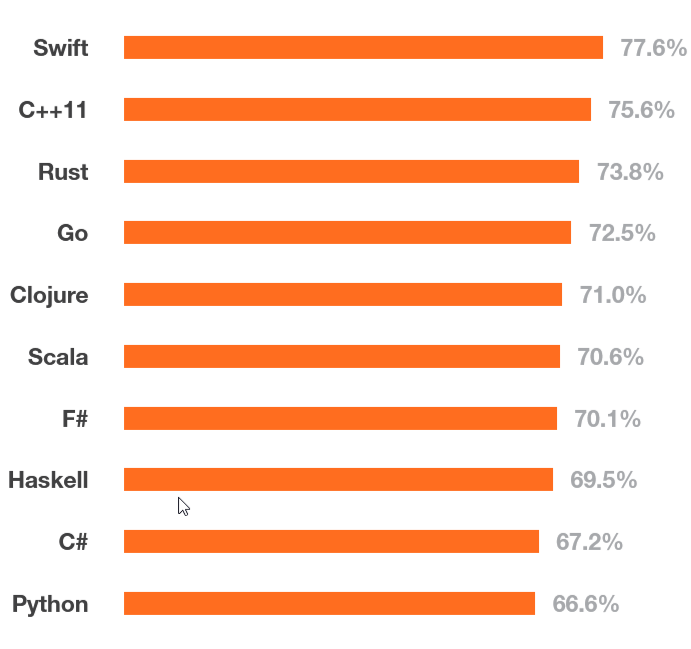
\includegraphics[width=0.90\linewidth]{Most.png}
	\caption{Most Loved Technologies, 2015 StackOverFlow Developer Survey \cite{moutidis2021community}}
\end{figure}

\textbf {Pros of Using Swift for iOS Native Development :} \cite{10.1145/3196398.3196428}
\begin{itemize}
	\item Rapid development process
	\item Easier to scale the product and the team
	\item Improved performance, speed of development, and safety
	\item Decreased memory footprint
	\item Interoperability with Objective-C
	\item Automatic memory management with ARC
	\item Full stack potential and cross-device support
	\item Vibrant open source community and learnability
\end{itemize}

\textbf {Cons of Using Swift Programming Language :} \cite{nayebi2017swift}
\begin{itemize}
	\item  The language is still quite young
	\item  Limited talent pool
	\item Poor interoperability with third-party tools and IDEs
	\item  Incomplete cross-platform support
	\item  Lack of support for earlier iOS versions
\end{itemize}

%-------------------------------------------------------------------------------------------------

 \section*{Conclusion}

In conclusion, SWIFT is a programming language developed by Apple Inc. to create applications for its operating system, iOS. This language was created with the primary goal of being more user-friendly and safer than other programming languages like Objective-C.

SWIFT offers many advantages over other programming languages, such as being more intuitive and easier to understand, reducing the likelihood of errors and providing a faster development time. SWIFT also offers seamless integration with Objective-C code, which makes it easy to switch from one language to another.

In terms of syntax, SWIFT offers a clean and straightforward syntax, making it easy to read and understand. This language also offers modern features such as generics, type inference, and optional types, which makes it more flexible and efficient. \cite{10.1145/3383219.3383237}

SWIFT also offers a comprehensive set of frameworks, libraries, and tools that developers can use to build sophisticated and robust applications. These tools include Xcode, Interface Builder, and a wide range of APIs that provide access to the various hardware and software features of the Apple ecosystem.

Another advantage of SWIFT is its compatibility with Apple's development ecosystem \cite{fojtik2020swift}. This language can be used with Apple's Cocoa and Cocoa Touch frameworks, which makes it possible to build native iOS applications. Developers can also use SWIFT with other Apple technologies such as Core Data, Core Graphics, and Grand Central Dispatch.

SWIFT has gained popularity since its release, with many developers worldwide adopting it as their preferred programming language. This popularity is due to the many benefits that SWIFT offers, such as being safer, easier to read, and more efficient than other programming languages.

However, SWIFT is not without its challenges. One of the main challenges facing SWIFT is its learning curve. Developers who are new to SWIFT may find it challenging to adapt to the syntax and features of the language. Another challenge facing SWIFT is its backward compatibility. Apple's frequent updates and changes to the language make it difficult for developers to maintain their codebase \cite{el2018methodology}.

Despite these challenges, SWIFT remains a powerful and versatile programming language that offers many advantages to developers. This language has revolutionized the way developers build applications for Apple's ecosystem and has provided a more modern, intuitive, and safer alternative to other programming languages\cite{el2018methodology}.

In conclusion, SWIFT is a significant milestone in the evolution of programming languages. Its clean syntax, modern features, and seamless integration with Apple's ecosystem make it a preferred choice for many developers. As technology continues to evolve, SWIFT will undoubtedly continue to grow and become an essential tool for developers worldwide \cite{latif2016cross}.


%----------------------------------------------------------------------------------------
%	BIBLIOGRAPHY
%----------------------------------------------------------------------------------------

\bibliographystyle{unsrt}

\bibliography{sample.bib}

%----------------------------------------------------------------------------------------

\end{document}
